\documentclass[tikz]{standalone}
\begin{document}
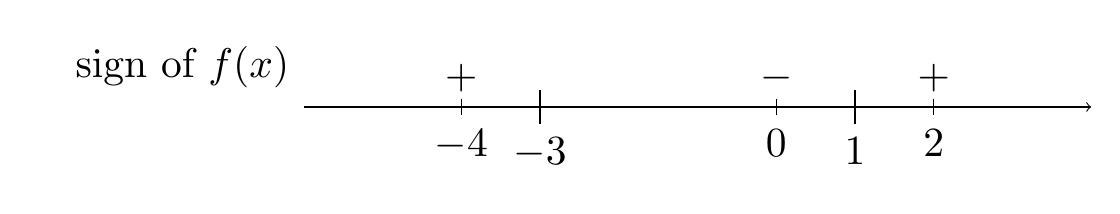
\begin{tikzpicture}[scale=1]
\draw[white,fill=white] (-9.5,-1) rectangle (4,1);
\draw[->](-6,0) -- (4,0) ;
\foreach \x in {-3, 1}
	\draw (\x, 6pt) -- (\x, -6pt) node[below, scale=1.5] {$\x$};
	
\node[above, scale=1.5] at (-4,0){$+$};
\node[above, scale=1.5] at (0,0){$-$};
\node[above, scale=1.5] at (2,0){$+$};

	\draw (-4, 3pt) -- (-4, -3pt) node[below, scale=1.5] {$-4$} ;
	\draw (0, 3pt) -- (0, -3pt) node[below, scale=1.5] {$0$} ;
	\draw (2, 3pt) -- (2, -3pt) node[below, scale=1.5] {$2$} ;

\node[left, scale=1.5] at (-6,0.5){sign of $f(x)$};
\end{tikzpicture} 
\end{document}
